%% Document template source: LaTeX2e template for FEUP's Project FE-UP
%% Document template author: jlopes@fe.up.pt
%% Template adapted

%% A alterar: <--ALTERAR-->

\documentclass[11pt,a4paper]{report}

%% Macros ----------------------------------------------------------------------
\newcommand{\school}{Instituto Superior de Engenharia de Lisboa}
\newcommand{\degree}{Licenciatura em Engenharia Eletrotécnica, Telecomunicações e Computadores}
\newcommand{\projisel}{Projeto ISEL 2023/24 --- LEETC}
\newcommand{\projtitle}{Computer Networks}
\newcommand{\projsubtitle}{Phase 2 - Connecting Devices}
\newcommand{\projteam}{Grupo LP-07}

%% Package ---------------------------------------------------------------------
\usepackage[T1]{fontenc}            % PS fonts
\usepackage[a4paper,left=25mm,right=25mm,top=25mm,bottom=25mm,headheight=6mm,footskip=12mm]{geometry}   % Document dimensions
\usepackage[english]{babel}         % [portuges]??
\usepackage[export]{adjustbox}      %
\usepackage[normalem]{ulem}         % various types of underlining
\usepackage[table,xcdraw]{xcolor}   % driver-independent color extensions
\usepackage[utf8]{inputenc}         % accents
\usepackage{amsmath}                % multi-line and other mathematical statements
\usepackage{array}                  % Images in tables
\usepackage{booktabs}
\usepackage{caption}                % rotating captions, sideways captions, etc.
\usepackage{chicago}                % Bibliography style
\usepackage{color}                  %
\usepackage{fancyhdr}               % Headers and footers
\usepackage{float}                  % tables and figures in the multi-column environment 
\usepackage{graphicx}               % 
\usepackage{hyperref}               % Hyper references
\usepackage{lastpage}               % 
\usepackage{lipsum}                 % loren dummy text
\usepackage{listings}               % Programming syntax
\usepackage{longtable}              % Tables continue in the next page
\usepackage{multicol}               % 
\usepackage{multirow}               % tabular cells spanning multiple rows
\usepackage{newtxtext,newtxmath}    % do not use CM fonts
\usepackage{paralist}
\usepackage{setspace}               % setting the spacing between lines
\usepackage{subcaption}             % for subfigures and the like

%% Package settings ------------------------------------------------------------
\graphicspath{{./images}}                           % {graphicx} - Images path % BY PHASE!!!
\selectlanguage{english}                            % {babel} - Language portuguese
\setlength{\columnsep}{3cm}                         % {multicol} - Column spacement
\definecolor{engineering}{rgb}{0.549,0.176,0.098}   % {color}
\definecolor{cloudwhite}{cmyk}{0,0,0,0.025}         % {color}
\definecolor{deepblue}{rgb}{0,0,0.5}                % {color}
\definecolor{deepred}{rgb}{0.6,0,0}                 % {color}
\definecolor{deepgreen}{rgb}{0,0.5,0}               % {color}
\setlength{\parindent}{0em}                         % {geometry}
\setlength{\parskip}{1ex}                           % {geometry}
\lstdefinestyle{pythoncode}                         % {listings} - Python syntax
{
    aboveskip=8mm,
    backgroundcolor=\color{cloudwhite},             
    basicstyle=\footnotesize\ttfamily,
    numbers=left,                                   % where to put the line-numbers
    belowskip=4mm,
    breakatwhitespace=false,                        % sets if automatic breaks should only happen at whitespace
    breaklines=true,                                % sets automatic line breaking
    captionpos=b,                                   % sets the caption-position to bottom
    escapeinside={\%*}{*)},                         % if you want to add a comment within your code
    float=htb,
    frame=tb,
    keepspaces=true,
    keywordstyle=\bfseries\color{deepblue},
    morekeywords={*,var,template,new}               % if you want to add more keywords to the set
    numbersep=8pt,                                  % how far the line-numbers are from the code
    numberstyle=\scriptsize\texttt,                 % the size of the fonts that are used for the line-numbers
    showspaces=false,                               % show spaces adding particular underscores
    showstringspaces=false,                         % underline spaces within strings
    showtabs=false,                                 % show tabs within strings adding particular underscores
    stepnumber=1,                                   % the step between two line-numbers. If it's 1 each line will be numbered
    stringstyle=\color{deepgreen},
    tabsize=2,                                      % sets default tabsize to 2 spaces
}
\lstdefinestyle{termoutputs}                        % {listings} - Python syntax
{
    aboveskip=8mm,
    backgroundcolor=\color{cloudwhite},             
    basicstyle=\scriptsize\ttfamily,
    numbers=left,                                   % where to put the line-numbers
    belowskip=4mm,
    breakatwhitespace=false,                        % sets if automatic breaks should only happen at whitespace
    breaklines=true,                                % sets automatic line breaking
    captionpos=b,                                   % sets the caption-position to bottom
    escapeinside={\%*}{*)},                         % if you want to add a comment within your code
    float=htb,
    frame=tb,
    keepspaces=true,
    keywordstyle=\bfseries\color{deepblue},
    morekeywords={*,var,template,new}               % if you want to add more keywords to the set
    numbersep=8pt,                                  % how far the line-numbers are from the code
    numberstyle=\scriptsize\texttt,                 % the size of the fonts that are used for the line-numbers
    showspaces=false,                               % show spaces adding particular underscores
    showstringspaces=false,                         % underline spaces within strings
    showtabs=false,                                 % show tabs within strings adding particular underscores
    stepnumber=1,                                   % the step between two line-numbers. If it's 1 each line will be numbered
    stringstyle=\color{deepgreen},
    tabsize=2,                                      % sets default tabsize to 2 spaces
}
\fancyhf{}                                          % {fancyhdr} clear off all default fancyhdr headers and footers
\lfoot{\small{\emph{\projtitle, \projsubtitle}}}    % {fancyhdr}
\rfoot{\small{\thepage\ / \pageref{LastPage}}}      % {fancyhdr}
\pagestyle{fancy}                                   % {fancyhdr} apply the fancy header style
\renewcommand{\headrulewidth}{0.0pt}                % {fancyhdr} no head rule
\renewcommand{\footrulewidth}{0.4pt}                % {fancyhdr}
\hypersetup{                                        % {hyperref}
    plainpages=false,
    pdfpagelayout=SinglePage,
    bookmarksopen=false,
    bookmarksnumbered=true,
    breaklinks=true,
    linktocpage,
    colorlinks=true,
    linkcolor=engineering,
    urlcolor=engineering,
    filecolor=engineering,
    citecolor=engineering,
    allcolors=engineering
}

%% Document start --------------------------------------------------------------
\begin{document}
    \pagenumbering{roman}\setcounter{page}{1}

%% Cover -----------------------------------------------------------------------
\begin{titlepage}
    \center

    \vspace*{-12mm}
    {\large \textbf{\textsc{\school}}}\\

    \vfill

    
\includegraphics[width=62mm]{logoisel}
    
    \vfill
    
    {\huge \textbf{\projtitle}}\\[6mm]
    {\Large \textbf{\projsubtitle}}\\
    
    \vfill
    
    \vfill
    
    {\Large \textbf{\projisel}}\\[12mm]
    
    {\Large \textbf{Coordination}}\\[4mm]
    {\large General: Carlos Meneses\hspace*{18mm}
            Course: Nuno Cruz}\\[6mm]
    
    {\Large \textbf{\projteam}}\\[4mm]
    {\large Supervisor: Luís Pires\hspace*{12mm}}\\[6mm]
    
    {\Large \textbf{Student}}\\[4mm]
    {\large Nuno Brito $<$A46948@alunos.isel.pt$>$}
    
    \vspace*{10mm}
    
    \renewcommand{\today}{May 5th 2024}
    \today
    
\end{titlepage}

%% TOC -------------------------------------------------------------------------
\tableofcontents

%% List of figures -------------------------------------------------------------
\listoffigures
\addcontentsline{toc}{chapter}{Figure list}

%% List of tables --------------------------------------------------------------
\listoftables
\addcontentsline{toc}{chapter}{Table list}

%% List of listings --------------------------------------------------------------
\lstlistoflistings
\addcontentsline{toc}{chapter}{Listings list}

%% Acronyms --------------------------------------------------------------------
\chapter*{Acronyms list}
    \addcontentsline{toc}{chapter}{Acronyms list}

    \begin{flushleft}
        \begin{tabular}{l p{0.8\linewidth}}
            API     & Application Programming Interface\\
            CLI     & Command Line Interface\\
            CMD     & Command Prompt\\
            GUI     & Graphical User Interface\\
            HTTP    & Hyper Text Transfer Protocol\\
            HTTPS   & Hyper Text Transfer Protocol Secure\\
            IP      & Internet Protocol\\
            IPv4    & Internet Protocol version 4\\
            IPv6    & Internet Protocol version 6\\
            LAN     & Local Area Network\\
            OS      & Operating System\\
            OSS     & openSUSE\\
            PC      & Personal Computer\\
            PHP     & PHP: Hypertext Preprocessor\\
            SSL     & Secure Sockets Layer\\
            TCP     & Transmission Control Protocol\\
            TLS     & Transport Layer Security\\
            TUI     & Terminal User Interface\\ % Not used yet
            UDP     & User Datagram Protocol\\
            VPN     & Virtual Private Network\\
            WWW     & World Wide Web\\
            XAMPP   & Cross-Platform, Apache, MySQL, PHP, and Perl
        \end{tabular}
    \end{flushleft}

%% Glossary --------------------------------------------------------------------
\chapter*{Glossary}
    \addcontentsline{toc}{chapter}{Glossary}

    \begin{description}
        \item[Apache2] \hfill \\
            An opensource HTTP web server.
        \item[Bit] \hfill \\
            A unit of information in computing and digital communications. The bit represents a logical state with one of two possible values, 0 or 1 (other representations such as \textit{true / false} are also valid).
        \item[Byte] \hfill \\
            Also a unit of digital information, consists of 8 bits.
        \item[Broadcast] \hfill \\
            A method of transferring a message to all recipients simultaneously.
        \item[Browser] \hfill \\
            A browser is a internet navigation software. It comes in multiple flavours, nowadays the big three are Microsoft Edge, Mozilla Firefox and Google Chrome.
        \item[Cisco Packet Tracer] \hfill \\
            A cross-platform visual network simulation tool.
        \item[Command Prompt] \hfill \\
            The default command-line interpreter for Windows operating systems.
        \item[Firewall] \hfill \\
            A barrier between networks. Controls inbound and outbound traffic.
        \item[Gateway] \hfill \\
            A network gateway provides a connection between networks and devices. Known as protocol translation gateways or mapping gateways, can perform protocol conversions to connect networks with different network protocol technologies.
        \item[LibreWolf] \hfill \\
            An internet browser based on Mozilla's Firefox. It's primary purpose is to allow privacy, and with it comes security. It achieves this by removing telemetry and data collection.
        \item[Linux] \hfill \\
            Open-source Unix-like operating systems based on the Linux kernel.
        \item[MariaDB] \hfill \\
            A community-developed fork of MySQL database server.
        \item[openSUSE Tumbleweed] \hfill \\
            An openSUSE (OSS) is an open-source community driven Linux-based distribuition sponsored by SUSE Software Solutions. Tumbleweed is a rolling release version allowing for up-to-date software releases.
        \item[Operating system] \hfill \\
            A program that manages a computer's resources from software to hardware.
        \item[Ping] \hfill \\
             A software utility used to test the reachability of a host on an IP network.
        \item[Tracert] \hfill \\
            Or \textbf{traceroute} in unix and linux systems, is a computer network diagnostic command for displaying possible routes and measuring transit delays of packets across an IP network.
        \item[Ipconfig] \hfill \\
            Or \textbf{ifconfig} in unix and linux systems, is a console application program that displays all current TCP/IP network configuration values.
        \item[Python] \hfill \\
            Python is a high-level programming language, object-oriented.
        \item[Perl] \hfill \\
            A high-level, general-purpose, interpreted, dynamic programming language
        \item[Rolling release distribuition] \hfill \\
            A distribuition where it's software release cycle is more frequent than those of Long Term Support (LTS). It's up to the Linux-based distribuitor to guarantee the testing of a package.
        \item[Router] \hfill \\
            A networking device that forwards data packets between computer networks, including internetworks such as the global Internet.
        \item[Switch] \hfill \\
            A networking hardware that connects devices on a computer network by using packet switching to receive and forward data to the destination device.
        \item[Socket] \hfill \\
            A network socket serves as an endpoint for sending and receiving data across the network.
        \item[Subnet Mask] \hfill \\
            Is a logical subdivision of an IP network.
        \item[Unix] \hfill \\
            Is a family of multitasking, multi-user computer operating systems that derive from the original AT\&T Unix.
        \item[VPN] \hfill \\
            A private network creating a secure connection between a device and a network.
        \item[Windows] \hfill \\
            Microsoft's operating system. First released in 1985 as a Graphical User Interface (GUI) for MS-DOS, continued to evolve with it's latest version being 11.
            Due to it's nature, it's not recommended for server production environment.
        \item[Wireshark] \hfill \\
            Wireshark is a network protocol analyser software. Allows traffic capture between a computer and a network.
        \item[XAMPP] \hfill \\
            A software package environment collection containing Apache2 webserver, MariaDB database, PHP and Perl.
    \end{description}

%% Chapter: introduction -------------------------------------------------------
\chapter{Introduction}
% display headers & footers
    \pagestyle{fancy}
    For phase 2 we were tasked to configure two local area networks using a router. By applying the principles of subnetting we can dimension our network pragmatically, keeping in check the assigned requirements, wasting only a minimal ammount of unallocated IP addresses.\\
    Since the next phases overlap in planning, the majority of information presented in this report will be used for the upcoming parts. Time is of essence, this little manuveur allowed us to save on time and energy since all the hard work is done.\\
    To better understand what we're dealing with we'll also explore a little bit about IP version 4, what it contains and how does it work. Concepts about routers, configuring our devices, taking advantage of switches and so on are also displayed in this phase.\\

% main page numbers with arabic numerals
    \pagenumbering{arabic}\setcounter{page}{1}

%% Chapter: phase 2 ------------------------------------------------------------
\chapter{Phase 2}
    \section{The IP Header}
        Before getting our hands-on business. Let's acquaintance our Internet Protocol (IP) friend, IPv4. To keep it simple we'll not touch IPv6.

        \begin{figure}[h]
            \centering
            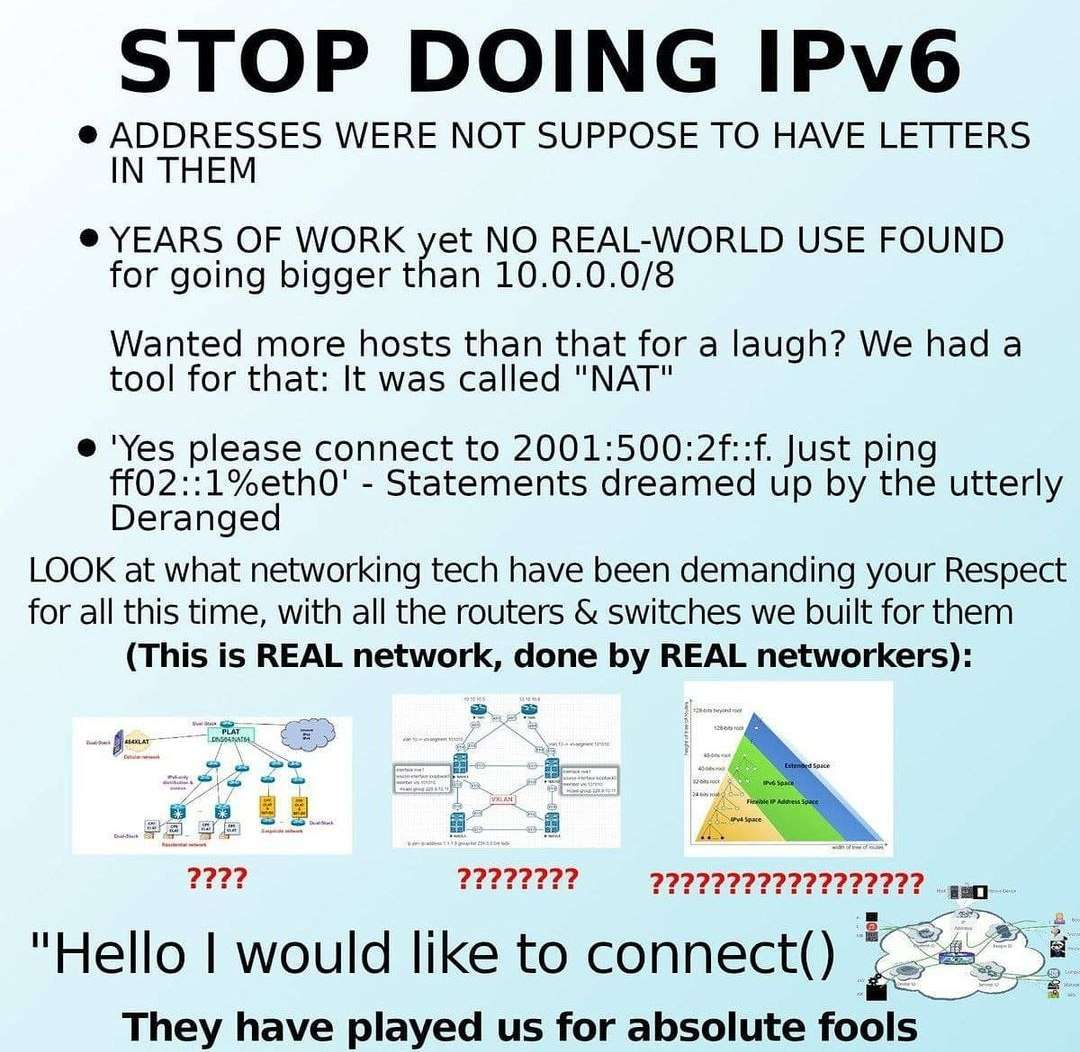
\includegraphics[scale=0.3]{stopdoingipv6} 
            \caption{Guess IPv4 is enough for everything}
            \label{fig:funnyipv6}
        \end{figure}
        \pagebreak

        Ok, now that we're at ease, we can explore the IP datagram.\\
        IP Datagram is the data transmitted over a network connection carried in messages, using specific formats as seen in table \ref{tab:ipdatagram}.

        \begin{center}
            \begin{longtable}{|ccclcccc|}
                \hline
                \multicolumn{1}{|c|}{\begin{tabular}[c]{@{}c@{}}Version\\ 4 bits\end{tabular}} & \multicolumn{1}{c|}{\begin{tabular}[c]{@{}c@{}}Header Length\\ 4bits\end{tabular}} & \multicolumn{2}{c|}{\begin{tabular}[c]{@{}c@{}}Type of Service\\ 8 bits\end{tabular}} & \multicolumn{4}{c|}{\begin{tabular}[c]{@{}c@{}}Total Length\\ 16 bits\end{tabular}}                                                                                                                                                                                                                                          \\ \hline
                \endfirsthead
                %
                \multicolumn{8}{c}%
                {{\bfseries Table \thetable\ continued from previous page}} \\
                \hline
                \multicolumn{1}{|c|}{\begin{tabular}[c]{@{}c@{}}Version\\ 4 bits\end{tabular}} & \multicolumn{1}{c|}{\begin{tabular}[c]{@{}c@{}}Header Length\\ 4bits\end{tabular}} & \multicolumn{2}{c|}{\begin{tabular}[c]{@{}c@{}}Type of Service\\ 8 bits\end{tabular}} & \multicolumn{4}{c|}{\begin{tabular}[c]{@{}c@{}}Total Length\\ 16 bits\end{tabular}}                                                                                                                                                                                                                                          \\ \hline
                \endhead
                %
                \multicolumn{4}{|c|}{\begin{tabular}[c]{@{}c@{}}Identification\\ 16 bits\end{tabular}}                                                                                                                                                                      & \multicolumn{1}{c|}{\begin{tabular}[c]{@{}c@{}}Reserved\\ 1 bit\end{tabular}} & \multicolumn{1}{c|}{\begin{tabular}[c]{@{}c@{}}Don't Fragment\\ 1 bit\end{tabular}} & \multicolumn{1}{c|}{\begin{tabular}[c]{@{}c@{}}More Fragment\\ 1 bit\end{tabular}} & \begin{tabular}[c]{@{}c@{}}Fragment Offset\\ 13 bits\end{tabular} \\ \hline
                \multicolumn{2}{|c|}{\begin{tabular}[c]{@{}c@{}}Time to Live\\ 8 bits\end{tabular}}                                                                                 & \multicolumn{2}{c|}{\begin{tabular}[c]{@{}c@{}}Protocol\\ 8 bits\end{tabular}}        & \multicolumn{4}{c|}{\begin{tabular}[c]{@{}c@{}}Header Checksum\\ 16 bits\end{tabular}}                                                                                                                                                                                                                                       \\ \hline
                \multicolumn{8}{|c|}{\begin{tabular}[c]{@{}c@{}}Source IP\\ 32 bits (4 Bytes)\end{tabular}}                                                                                                                                                                                                                                                                                                                                                                                                                                                                                                \\ \hline
                \multicolumn{8}{|c|}{\begin{tabular}[c]{@{}c@{}}Destination IP\\ 32 bits (4 Bytes)\end{tabular}}                                                                                                                                                                                                                                                                                                                                                                                                                                                                                           \\ \hline
                \multicolumn{8}{|c|}{\begin{tabular}[c]{@{}c@{}}Option\\ 0 - 40 Bytes\end{tabular}}                                                                                                                                                                                                                                                                                                                                                                                                                                                                                                        \\ \hline
                \multicolumn{8}{|c|}{\begin{tabular}[c]{@{}c@{}}DATA\\ 20 Bytes - 65536 Bytes\end{tabular}}                                                                                                                                                                                                                                                                                                                                                                                                                                                                                                \\ \hline
                \caption{IPv4 datagram dissected}
                \label{tab:ipdatagram}\\
            \end{longtable}
        \end{center}

        Each line, excluding \textit{option} and \textit{data}, have 32 bits (4 Bytes) of size.\\
        Breaking down each part of the protocol we can see the following:\\

        \begin{compactitem}
            \item \textbf{Version:} the IP version, 4 for IPv4.
            \item \textbf{Header Length:} the number of 32 bits words in the header with a minimum value of 5 and a maximum value of 15.
            \item \textbf{Type of service:} low delay, high throughput or reliability.
            \item \textbf{Total Length:} header plus data length with minimum value of 20 Bytes and a maximum value of 65535 Bytes.
                32 bits in total (4 Bytes)
            \item \textbf{Identification:} a unique packet id.
            \item \textbf{Flags}
            \begin{compactitem}
                \item \textbf{Reserved bit:} must be zero.
                \item \textbf{Don't Fragment}
                \item \textbf{More Fragment}
            \end{compactitem}
        \item \textbf{Fragment offset:} number of data Bytes ahead of the particular fragment in the particular datagram.
                32 bits in total (4 Bytes)
            \item \textbf{Time to live:} datagram lifetime.
            \item \textbf{Protocol:} name of the protocol.
            \item \textbf{Header checksum:} allows error checking in the header.
                32 bits in total (4 Bytes)
            \item \textbf{Source IP}
            \item \textbf{Destination IP}
            \item \textbf{Option:} optional information for network administrators.
        \end{compactitem}

    \section{Connecting two devices with a switch}
        This first part is very simple. There are two devices (PC0 and Laptop0) connected to a switch and their network starts with 192.168.\textbf{\textit{GROUP NUMBER}}.0.\\
        Therefore:

        \begin{compactitem}
            \item Group: 7 [192.168.7.0/24]
            \item Laptop0  [192.168.7.1]
            \item PC0      [192.168.7.2]
        \end{compactitem}

        After applying the configuration we must run a set of commands to test our network.
        \begin{itemize}
            \item Ping: to test connectivity between devices over IP.
            \item Tracert: diagnostic command for displaying possible routes, also measures transit delay of packages across IP.
            \item Ipconfig: console application program of some computer operating systems that displays all current TCP/IP network configuration values. Unix and linux equivalent is \textit{ifconfig}.
        \end{itemize}

    \subsection{Simulating a network using Cisco Packet Tracer}
        For this project Cisco Packet Tracer will be our main tool. Using the Command Prompt (CMD) in each device, we'll simulate all referenced commands in the network.\\
        So let's get into this magnificient world, starting with these steps:\\
        \begin{flushleft}
            \begin{center}
                \begin{longtable}{ m{5cm} l }
                    \textbf{Steps} & \textbf{Example} \\
                    \hline
                    \endfirsthead
                    \multicolumn{2}{c}%
                    {{\bfseries Table \thetable\ continued from previous page}} \\
                    \textbf{Steps} & \textbf{Example} \\
                    \hline
                    \endhead
                    \hline Continued on next page \\
                    \endfoot
                    \endlastfoot

                    To configure the IP on a device we must \textbf{single-click} in the intended device (1), go to the \textit{desktop tab} (2) and select \textit{IP Configuration} (3).                                                                                                      & 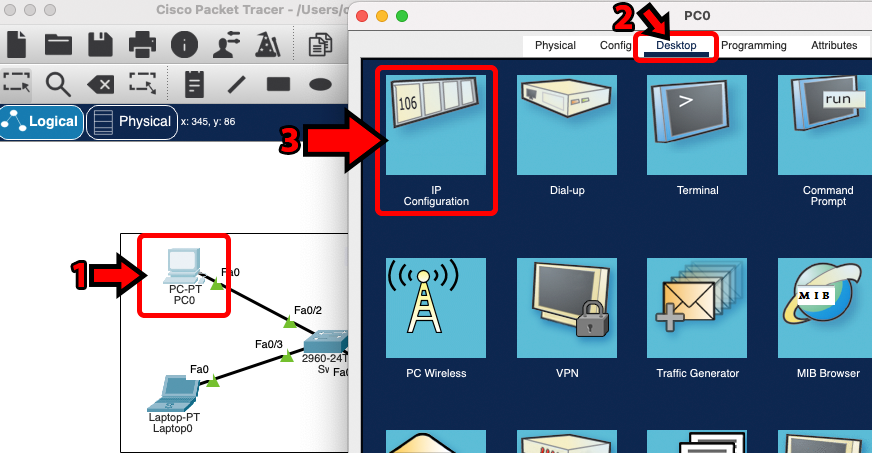
\includegraphics[scale=0.35,valign=c]{p1-connectingdevices/CiscoPacketTracer_configIP} \\ \hline
                    Now we configure our devices according to the required addresses.                                                                                                                                                                                                           & 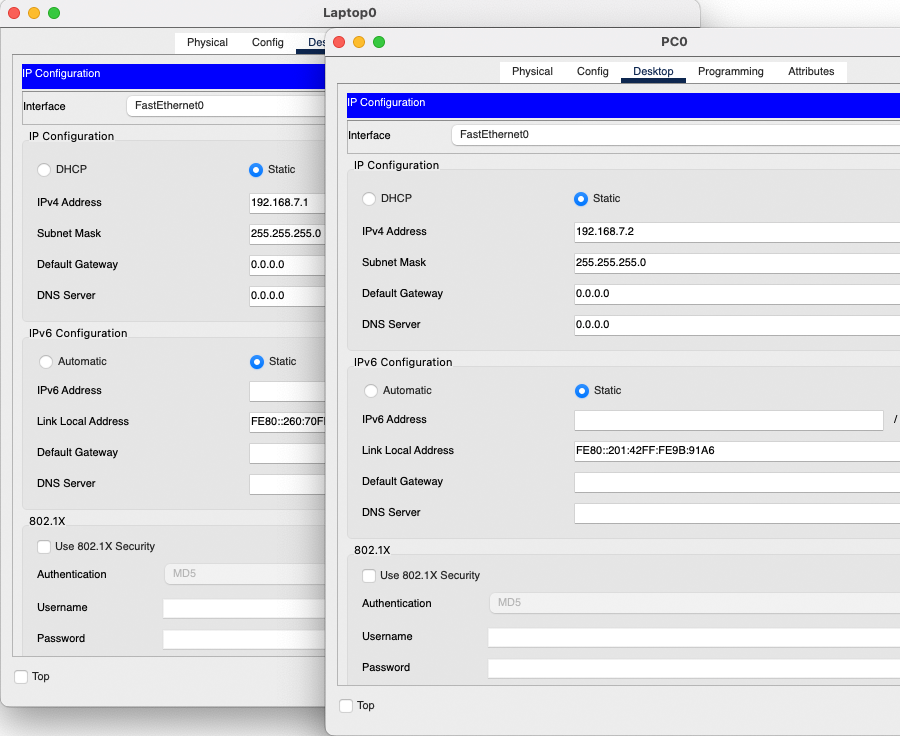
\includegraphics[scale=0.34,valign=c]{p1-connectingdevices/Laptop0PC0_ip} \\ \hline
                    To test the connection we select a device by \textbf{single-clicking} it (1), go to the \textit{desktop tab} (2) and select \textit{Command Prompt} (3).                                                                                                                    & 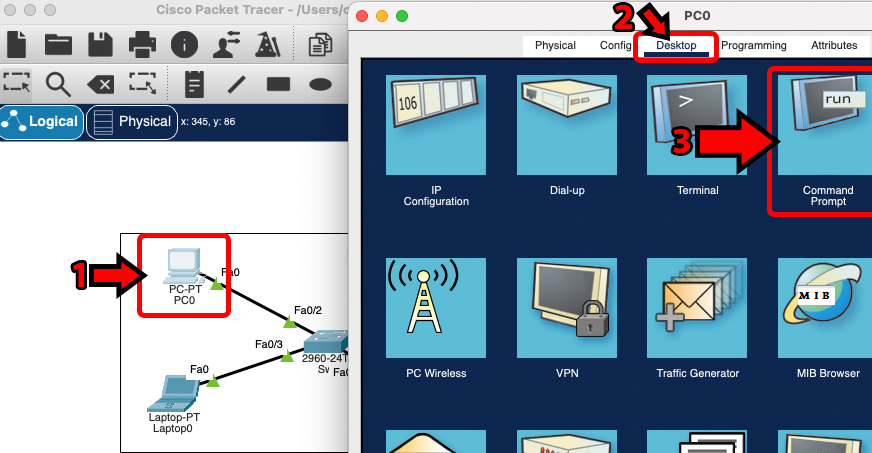
\includegraphics[scale=0.35,valign=c]{p1-connectingdevices/CiscoPacketTracer_cmdOutput} \\ \hline
                    We start by running \textit{arp -a} command, no prior discovery was made so the arp table will be empty. Then we'll \textit{ping} our other device. Run the \textit{arp -a} command again and we'll see it populated. If we do a \textit{tracert} there won't be any hops.    & 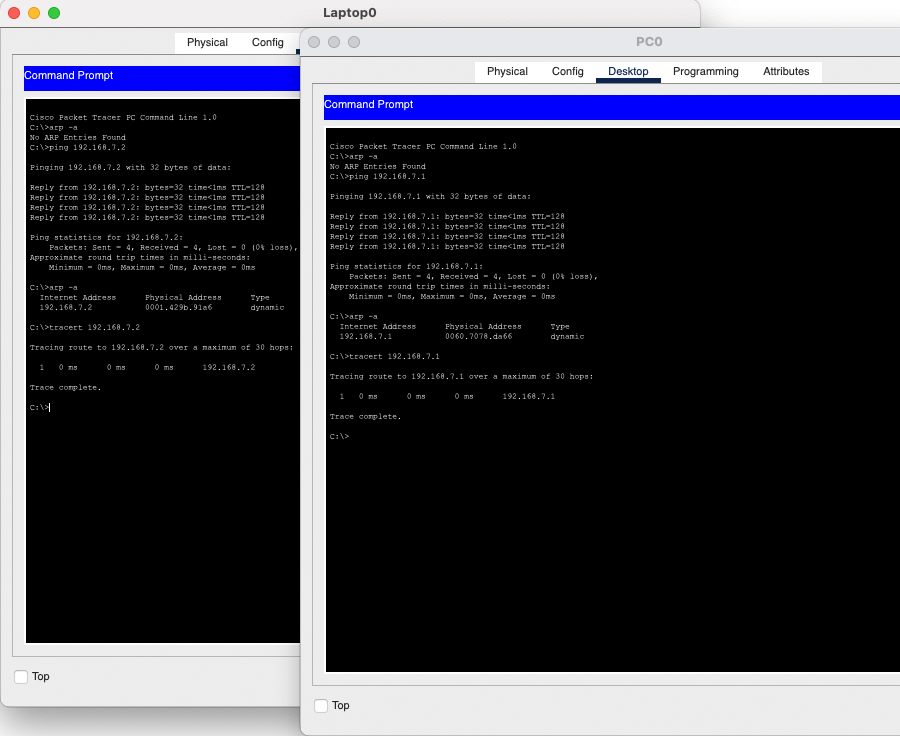
\includegraphics[scale=0.34,valign=c]{p1-connectingdevices/Laptop0PC0_cmd} \\ \hline

                    \caption{Cisco Packet Tracer guide}
                    \label{tab:cptg}
                \end{longtable}
            \end{center}
        \end{flushleft}

        And to supplement the output images, below are the text versions:
        \lstset{style=termoutputs}
        \lstinputlisting[
            language={},
            caption={PC0 CMD output},
            label={lst:pc0cmdoutp1}
        ]{./outputs/p1-connectingdevices/PC0.txt}
        \lstinputlisting[
            language={},
            caption={Laptop0 CMD output},
            label={lst:laptop0cmdoutp1}
        ]{./outputs/p1-connectingdevices/Laptop0.txt}

        \begin{quote}
            \textbf{Question:} How can a PC know if it is connected to a switch? Is traceroute useful in this situation? \\
            \\
            \textbf{Answer:}
            If a device is connected to a switch, the arp table will include both devices IP addresses after a ping to each other. However, if connected to a router (as we'll see in the next section), they we'll only include their gateways IP addresses.\\
            Traceroute isn't very useful here. It only shows hops in a routed network path (layer 3). Layer 2 devices, such as switches, won't show up since they receive and forward ethernet frames.\\
        \end{quote}

    \section{Connecting two LANs with a router}
        \begin{figure}[h]
            \centering
            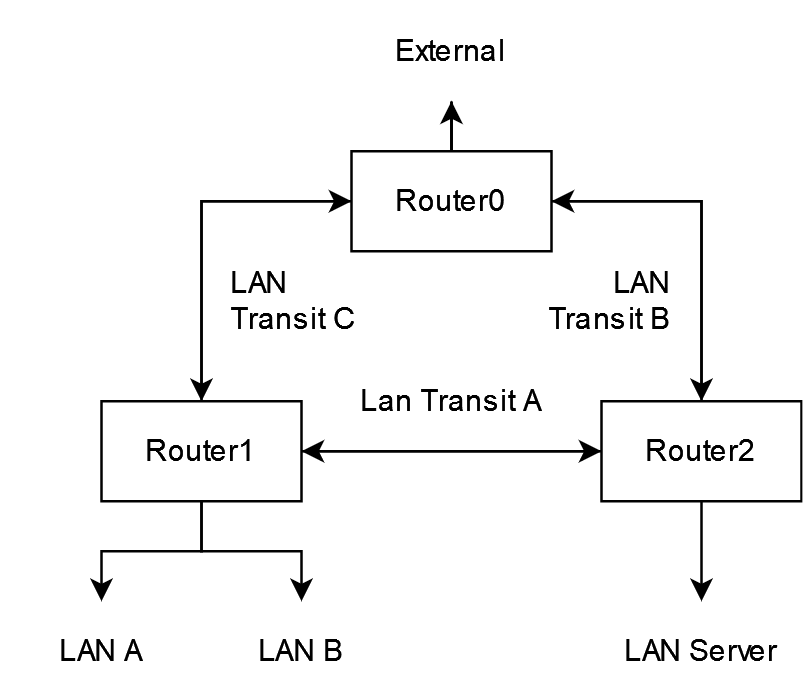
\includegraphics[scale=0.40,valign=c]{diagramL250}
            \caption{Part 2 network diagram}
            \label{fig:p2netdiag}
        \end{figure}

        Connecting to devices was pretty straight forward. Now comes the expected progress. What follows next tackles a network approach paramount for the next four phases.\\
            \[
                Clients_{LAN_A} = max\left(20, \left(\sum_{k=0}^n studentnumber_k\right)mod 100\right)\quad <=> 
                Clients_{LAN_A} = 48\quad
            \] \\
            \[
                Clients_{LAN_B} = \frac{Clients_{LAN_A}}{2}\quad <=>
                Clients_{LAN_B} = 27\quad
            \]\\

        Using the required mathmatical equations, provided in the project, we reach the conclusions presented in the following tables.\\

        \begin{center}
            \begin{longtable}{rlcccccccccccccccc}
                \hline
                \multicolumn{1}{c}{}                                                                                     & \textbf{}             & \multicolumn{16}{c}{\textbf{IP}}                                                                                                                                                                                                                                                                                                                                                                                                                                                                                  \\ \cline{3-18} 
                \multicolumn{1}{c}{\multirow{-2}{*}{\textbf{Subnet}}}                                                    &                       & \cellcolor[HTML]{C09FE5}0 & \cellcolor[HTML]{C09FE5}3 & \cellcolor[HTML]{C09FE5}4 & \cellcolor[HTML]{C09FE5}7 & \cellcolor[HTML]{C09FE5}8 & \cellcolor[HTML]{C09FE5}11 & \cellcolor[HTML]{C09FE5}12 & \cellcolor[HTML]{C09FE5}15 & \cellcolor[HTML]{BFBFBF}16      & \cellcolor[HTML]{BFBFBF}31      & \cellcolor[HTML]{FFD966}32      & \cellcolor[HTML]{FFD966}63      & \cellcolor[HTML]{A9D08E}64      & \cellcolor[HTML]{A9D08E}127     & \cellcolor[HTML]{F4B084}128      & \cellcolor[HTML]{F4B084}255     \\ \cline{1-1} \cline{3-18} 
                \endfirsthead
                %
                \multicolumn{18}{c}%
                {{\bfseries Table \thetable\ continued from previous page}} \\
                \hline
                \multicolumn{1}{c}{}                                                                                     & \textbf{}             & \multicolumn{16}{c}{\textbf{IP}}                                                                                                                                                                                                                                                                                                                                                                                                                                                                                  \\ \cline{3-18} 
                \multicolumn{1}{c}{\multirow{-2}{*}{\textbf{Subnet}}}                                                    &                       & \cellcolor[HTML]{C09FE5}0 & \cellcolor[HTML]{C09FE5}3 & \cellcolor[HTML]{C09FE5}4 & \cellcolor[HTML]{C09FE5}7 & \cellcolor[HTML]{C09FE5}8 & \cellcolor[HTML]{C09FE5}11 & \cellcolor[HTML]{C09FE5}12 & \cellcolor[HTML]{C09FE5}15 & \cellcolor[HTML]{BFBFBF}16      & \cellcolor[HTML]{BFBFBF}31      & \cellcolor[HTML]{FFD966}32      & \cellcolor[HTML]{FFD966}63      & \cellcolor[HTML]{A9D08E}64      & \cellcolor[HTML]{A9D08E}127     & \cellcolor[HTML]{F4B084}128      & \cellcolor[HTML]{F4B084}255     \\ \cline{1-1} \cline{3-18} 
                \endhead
                %
                \cline{1-1} \cline{3-18}
                \endfoot
                %
                \endlastfoot
                %
                \textbf{/25}                                                                                             &                       &                           &                           &                           &                           &                           &                            &                            &                            &                                 &                                 &                                 &                                 &                                 &                                 & \cellcolor[HTML]{F4B084}         & \cellcolor[HTML]{F4B084}        \\
                \textbf{/26}                                                                                             &                       &                           &                           &                           &                           &                           &                            &                            &                            &                                 &                                 &                                 &                                 & \cellcolor[HTML]{A9D08E}        & \cellcolor[HTML]{A9D08E}        &                                  &                                 \\
                \textbf{/27}                                                                                             &                       &                           &                           &                           &                           &                           &                            &                            &                            &                                 &                                 & \cellcolor[HTML]{FFD966}        & \cellcolor[HTML]{FFD966}        &                                 &                                 &                                  &                                 \\
                \textbf{/28}                                                                                             &                       &                           &                           &                           &                           &                           &                            &                            &                            & \cellcolor[HTML]{BFBFBF}        & \cellcolor[HTML]{BFBFBF}        &                                 &                                 &                                 &                                 &                                  &                                 \\
                \textbf{/30}                                                                                             &                       &                           &                           &                           &                           &                           &                            & \cellcolor[HTML]{C09FE5}   & \cellcolor[HTML]{C09FE5}   &                                 &                                 &                                 &                                 &                                 &                                 &                                  &                                 \\
                \textbf{/30}                                                                                             &                       &                           &                           &                           &                           & \cellcolor[HTML]{C09FE5}  & \cellcolor[HTML]{C09FE5}   &                            &                            &                                 &                                 &                                 &                                 &                                 &                                 &                                  &                                 \\
                \textbf{/30}                                                                                             &                       &                           &                           & \cellcolor[HTML]{C09FE5}  & \cellcolor[HTML]{C09FE5}  &                           &                            &                            &                            &                                 &                                 &                                 &                                 &                                 &                                 &                                  &                                 \\
                \textbf{/30}                                                                                             &                       & \cellcolor[HTML]{C09FE5}  & \cellcolor[HTML]{C09FE5}  &                           &                           &                           &                            &                            &                            &                                 &                                 &                                 &                                 &                                 &                                 &                                  &                                 \\ \cline{1-1} \cline{3-18} 
                                                                                                                         & \multicolumn{1}{l|}{} & \multicolumn{2}{l}{\cellcolor[HTML]{C09FE5}/30}       & \multicolumn{2}{c}{\cellcolor[HTML]{C09FE5}/30}       & \multicolumn{2}{c}{\cellcolor[HTML]{C09FE5}/30}        & \multicolumn{2}{c}{\cellcolor[HTML]{C09FE5}/30}         & \multicolumn{2}{c}{\cellcolor[HTML]{BFBFBF}}                      & \multicolumn{2}{c}{\cellcolor[HTML]{FFD966}}                      & \multicolumn{2}{c}{\cellcolor[HTML]{A9D08E}}                      & \multicolumn{2}{c|}{\cellcolor[HTML]{F4B084}}                      \\
                                                                                                                         & \multicolumn{1}{l|}{} & \multicolumn{4}{l}{/29}                                                                                       & \multicolumn{4}{c}{}                                                                                             & \multicolumn{2}{c}{\cellcolor[HTML]{BFBFBF}}                      & \multicolumn{2}{c}{\cellcolor[HTML]{FFD966}}                      & \multicolumn{2}{c}{\cellcolor[HTML]{A9D08E}}                      & \multicolumn{2}{c|}{\cellcolor[HTML]{F4B084}}                      \\
                                                                                                                         & \multicolumn{1}{l|}{} & \multicolumn{8}{l}{\cellcolor[HTML]{BFBFBF}/28}                                                                                                                                                                                  & \multicolumn{2}{c}{\multirow{-3}{*}{\cellcolor[HTML]{BFBFBF}/28}} & \multicolumn{2}{c}{\cellcolor[HTML]{FFD966}}                      & \multicolumn{2}{c}{\cellcolor[HTML]{A9D08E}}                      & \multicolumn{2}{c|}{\cellcolor[HTML]{F4B084}}                      \\
                                                                                                                         & \multicolumn{1}{l|}{} & \multicolumn{10}{l}{\cellcolor[HTML]{FFD966}/27}                                                                                                                                                                                                                                                     & \multicolumn{2}{c}{\multirow{-4}{*}{\cellcolor[HTML]{FFD966}/27}} & \multicolumn{2}{c}{\cellcolor[HTML]{A9D08E}}                      & \multicolumn{2}{c|}{\cellcolor[HTML]{F4B084}}                      \\
                                                                                                                         & \multicolumn{1}{l|}{} & \multicolumn{12}{l}{\cellcolor[HTML]{A9D08E}/26}                                                                                                                                                                                                                                                                                                                         & \multicolumn{2}{c}{\multirow{-5}{*}{\cellcolor[HTML]{A9D08E}/26}} & \multicolumn{2}{c|}{\cellcolor[HTML]{F4B084}}                      \\
                                                                                                                         & \multicolumn{1}{l|}{} & \multicolumn{14}{l}{\cellcolor[HTML]{F4B084}/25}                                                                                                                                                                                                                                                                                                                                                                                             & \multicolumn{2}{c|}{\multirow{-6}{*}{\cellcolor[HTML]{F4B084}/25}} \\
                \multirow{-7}{*}{\textbf{\begin{tabular}[c]{@{}r@{}}Subnet\\      visual\\      portrayal\end{tabular}}} & \multicolumn{1}{l|}{} & \multicolumn{16}{l|}{\cellcolor[HTML]{00B0F0}/24}                                                                                                                                                                                                                                                                                                                                                                                                                                                                 \\ \cline{1-1} \cline{3-18} 
                \caption{Visual LAN allocation}
                \label{tab:visuallanalloc}\\
            \end{longtable}
        \end{center}

        \begin{center}
            \begin{longtable}{lllllll}
                \hline
                                                               & \textbf{Network}           & \textbf{Usable IPs} & \textbf{Router} & \multicolumn{1}{c}{\textbf{Broadcast}} & \multicolumn{1}{c}{\textbf{Subnet Mask}} &                                      \\ \cline{2-5}
                \multirow{-2}{*}{\textbf{Name}}                & \multicolumn{4}{c}{192.168.7.}                                                                              & \multicolumn{1}{c}{255.255.255.}         & \multirow{-2}{*}{\textbf{Populated}} \\ \hline
                \endfirsthead
                %
                \multicolumn{7}{c}%
                {{\bfseries Table \thetable\ continued from previous page}} \\
                \hline
                                                               & \textbf{Network}           & \textbf{Usable IPs} & \textbf{Router} & \multicolumn{1}{c}{\textbf{Broadcast}} & \multicolumn{1}{c}{\textbf{Subnet Mask}} &                                      \\ \cline{2-5}
                \multirow{-2}{*}{\textbf{Name}}                & \multicolumn{4}{c}{192.168.7.}                                                                              & \multicolumn{1}{c}{255.255.255.}         & \multirow{-2}{*}{\textbf{Populated}} \\ \hline
                \endhead
                %
                \hline
                \endfoot
                %
                \endlastfoot
                %
                \cellcolor[HTML]{F4B084}\textbf{LAN Server}    & 128                        & 129 - 253           & 254             & 255                                    & 128                                      & 126                                  \\
                \cellcolor[HTML]{A9D08E}\textbf{LAN A}         & 64                         & 65 - 125            & 126             & 127                                    & 192                                      & 48                                   \\
                \cellcolor[HTML]{FFD966}\textbf{LAN B}         & 32                         & 33 - 61             & 62              & 63                                     & 224                                      & 27                                   \\ \hline
                                                               & \cellcolor[HTML]{BFBFBF}16 & 17 - 31             &                 & 32                                     &                                          & 0                                    \\
                \multirow{-2}{*}{\textbf{Unused remaining}}    & \cellcolor[HTML]{C09FE5}12 & 13 - 14             &                 & 15                                     &                                          & 0                                    \\ \hline
                \cellcolor[HTML]{C09FE5}\textbf{LAN Transit C} & 8                          & 9 - 10              &                 & 11                                     & 252                                      & 2                                    \\
                \cellcolor[HTML]{C09FE5}\textbf{LAN Transit B} & 4                          & 5 - 6               &                 & 7                                      & 252                                      & 2                                    \\
                \cellcolor[HTML]{C09FE5}\textbf{LAN Transit A} & 0                          & 1 - 2               &                 & 3                                      & 252                                      & 2                                    \\ \hline
                \caption{LAN allocation table}
                \label{tab:lanalloctable}\\
            \end{longtable}
        \end{center}

        \begin{center}
            \begin{longtable}{@{}llllll@{}}
                \toprule
                \multicolumn{1}{c}{\multirow{2}{*}{\textbf{Name}}} & \multicolumn{1}{c}{\multirow{2}{*}{\textbf{Ports Link}}} & \multicolumn{1}{c}{\multirow{2}{*}{\textbf{Network}}} & \multicolumn{1}{c}{\multirow{2}{*}{\textbf{IP}}} & \multicolumn{1}{c}{\multirow{2}{*}{\textbf{Subnet Mask}}} & \multicolumn{1}{c}{\multirow{2}{*}{\textbf{Gateway}}} \\
                \multicolumn{1}{c}{}                               & \multicolumn{1}{c}{}                                     & \multicolumn{1}{c}{}                                  & \multicolumn{1}{c}{}                             & \multicolumn{1}{c}{}                                      & \multicolumn{1}{c}{}                                  \\* \midrule
                \endfirsthead
                %
                \multicolumn{6}{c}%
                {{\bfseries Table \thetable\ continued from previous page}} \\
                \toprule
                \multicolumn{1}{c}{\multirow{2}{*}{\textbf{Name}}} & \multicolumn{1}{c}{\multirow{2}{*}{\textbf{Ports Link}}} & \multicolumn{1}{c}{\multirow{2}{*}{\textbf{Network}}} & \multicolumn{1}{c}{\multirow{2}{*}{\textbf{IP}}} & \multicolumn{1}{c}{\multirow{2}{*}{\textbf{Subnet Mask}}} & \multicolumn{1}{c}{\multirow{2}{*}{\textbf{Gateway}}} \\
                \multicolumn{1}{c}{}                               & \multicolumn{1}{c}{}                                     & \multicolumn{1}{c}{}                                  & \multicolumn{1}{c}{}                             & \multicolumn{1}{c}{}                                      & \multicolumn{1}{c}{}                                  \\* \midrule
                \endhead
                %
                \bottomrule
                \endfoot
                %
                \endlastfoot
                %
                \textbf{PC0}                                       & Fa0 - Sw0 Fa0/2                                          & \multirow{2}{*}{LAN A}                                & 192.168.7.65                                     & 255.255.255.192                                           & 192.168.7.126                                         \\
                \textbf{Laptop0}                                   & Fa0 - Sw0 Fa0/3                                          &                                                       & 192.168.7.66                                     & 255.255.255.192                                           & 192.168.7.126                                         \\* \midrule
                \textbf{PC1}                                       & Fa0 - Sw1 Fa0/2                                          & \multirow{2}{*}{LAN B}                                & 192.168.7.33                                     & 255.255.255.224                                           & 192.168.7.62                                          \\
                \textbf{Laptop1}                                   & Fa0 - Sw1 Fa0/3                                          &                                                       & 192.168.7.34                                     & 255.255.255.224                                           & 192.168.7.62                                          \\* \midrule
                \multirow{3}{*}{\textbf{R0}}                       & Fa5/0 - R1 Fa5/0                                         & LAN Transit B                                         & 192.168.7.5                                      & 255.255.255.252                                           &                                                       \\
                                                                   & Fa4/0 - R2 Fa4/0                                         & LAN Transit C                                         & 192.168.7.9                                      & 255.255.255.252                                           &                                                       \\
                                                                   & Fa0/0                                                    & External                                              &                                                  &                                                           &                                                       \\* \midrule
                \multirow{4}{*}{\textbf{R1}}                       & Fa4/0 - R2 Fa5/0                                         & LAN Transit A                                         & 192.168.7.1                                      & 255.255.255.252                                           &                                                       \\
                                                                   & Fa5/0 - R1 Fa4/0                                         & LAN Transit B                                         & 192.168.7.6                                      & 255.255.255.252                                           &                                                       \\
                                                                   & Fa0/0 - Sw0 Fa0/1                                        & LAN A                                                 & 192.168.7.126                                    & 255.255.255.192                                           &                                                       \\
                                                                   & Fa1/0 - Sw1 Fa0/1                                        & LAN B                                                 & 192.168.7.62                                     & 255.255.255.224                                           &                                                       \\* \midrule
                \multirow{3}{*}{\textbf{R2}}                       & Fa5/0 - R1 Fa4/0                                         & LAN Transit A                                         & 192.168.7.2                                      & 255.255.255.252                                           &                                                       \\
                                                                   & Fa4/0 - R0 Fa4/0                                         & LAN Transit C                                         & 192.168.7.10                                     & 255.255.255.252                                           &                                                       \\
                                                                   & Fa0/0 - Sw2 Fa0/4                                        & LAN Server                                            & 192.168.7.254                                    & 255.255.255.128                                           &                                                       \\* \midrule
                \textbf{DHCP Server}                               & Fa0 - Sw2 Fa0/3                                          & \multirow{3}{*}{LAN Server}                           & 192.168.7.129                                    & 255.255.255.128                                           & 192.168.7.254                                         \\
                \textbf{DNS Server}                                & Fa0 - Sw2 Fa0/2                                          &                                                       & 192.168.7.130                                    & 255.255.255.128                                           & 192.168.7.254                                         \\
                \textbf{HTTP Server}                               & Fa0 - Sw2 Fa0/1                                          &                                                       & 192.168.7.131                                    & 255.255.255.128                                           & 192.168.7.254                                         \\* \midrule
                \multirow{3}{*}{\textbf{Sw0}}                      & Fa0/1 - R1 Fa0/0                                         & \multirow{3}{*}{LAN A}                                & \multicolumn{1}{c}{}                             & \multicolumn{1}{c}{}                                      & \multicolumn{1}{c}{}                                  \\
                                                                   & Fa0/2 - PC0                                              &                                                       & \multicolumn{1}{c}{}                             & \multicolumn{1}{c}{}                                      & \multicolumn{1}{c}{}                                  \\
                                                                   & Fa0/3 - Laptop0                                          &                                                       & \multicolumn{1}{c}{}                             & \multicolumn{1}{c}{}                                      & \multicolumn{1}{c}{}                                  \\* \midrule
                \multirow{3}{*}{\textbf{Sw1}}                      & Fa0/1 - R1 Fa1/0                                         & \multirow{3}{*}{LAN B}                                & \multicolumn{1}{c}{}                             & \multicolumn{1}{c}{}                                      & \multicolumn{1}{c}{}                                  \\
                                                                   & Fa0/2 - PC1                                              &                                                       & \multicolumn{1}{c}{}                             & \multicolumn{1}{c}{}                                      & \multicolumn{1}{c}{}                                  \\
                                                                   & Fa0/3 - Laptop1                                          &                                                       & \multicolumn{1}{c}{}                             & \multicolumn{1}{c}{}                                      & \multicolumn{1}{c}{}                                  \\* \midrule
                \multirow{4}{*}{\textbf{Sw2}}                      & Fa0/1 - HTTP                                             & \multirow{4}{*}{LAN Server}                           & \multicolumn{1}{c}{}                             & \multicolumn{1}{c}{}                                      & \multicolumn{1}{c}{}                                  \\
                                                                   & Fa0/2 - DNS                                              &                                                       & \multicolumn{1}{c}{}                             & \multicolumn{1}{c}{}                                      & \multicolumn{1}{c}{}                                  \\
                                                                   & Fa0/3 - DHCP                                             &                                                       & \multicolumn{1}{c}{}                             & \multicolumn{1}{c}{}                                      & \multicolumn{1}{c}{}                                  \\
                                                                   & Fa0/4 - R2 Fa0/0                                         &                                                       & \multicolumn{1}{c}{}                             & \multicolumn{1}{c}{}                                      & \multicolumn{1}{c}{}                                  \\* \bottomrule
                \caption{IP configuration table}
                \label{tab:deviceiptable}\\
                \end{longtable}
        \end{center}

        Instead of planning for each phase and re-assigning the entire network, it was opted to fully outline every subnet and device in a pramatic manner.\\
        However, here we'll focus on router \textbf{\textit{R1}}, and the respective networks, \textbf{\textit{LAN A}} and \textbf{\textit{LAN B}}.\\

        Once again, \textbf{Cisco Packet Tracer} to the help:

        \begin{flushleft}
                \begin{center}
                    \begin{longtable}{ m{5cm} l }
                        \textbf{Steps} & \textbf{Example} \\
                        \hline
                        \endfirsthead
                        \multicolumn{2}{c}%
                        {{\bfseries Table \thetable\ continued from previous page}} \\
                        \textbf{Steps} & \textbf{Example} \\
                        \hline
                        \endhead
                        \hline Continued on next page \\
                        \endfoot
                        \endlastfoot

                        To configure the IP on a device we must \textbf{single-click} in the intended device (1), go to the \textit{desktop tab} (2) and select \textit{IP Configuration} (3).                                                                                                                                                                                                                      & 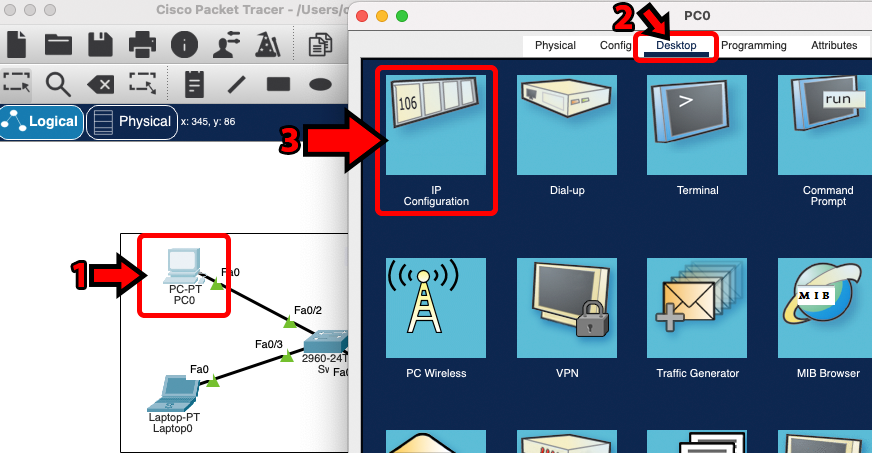
\includegraphics[scale=0.35 ,valign=c]{p1-connectingdevices/CiscoPacketTracer_configIP}   \\ \hline
                        Configure Laptop0 and PC0 computers accordingly to our results.                                                                                                                                                                                                                                                                                                                             & 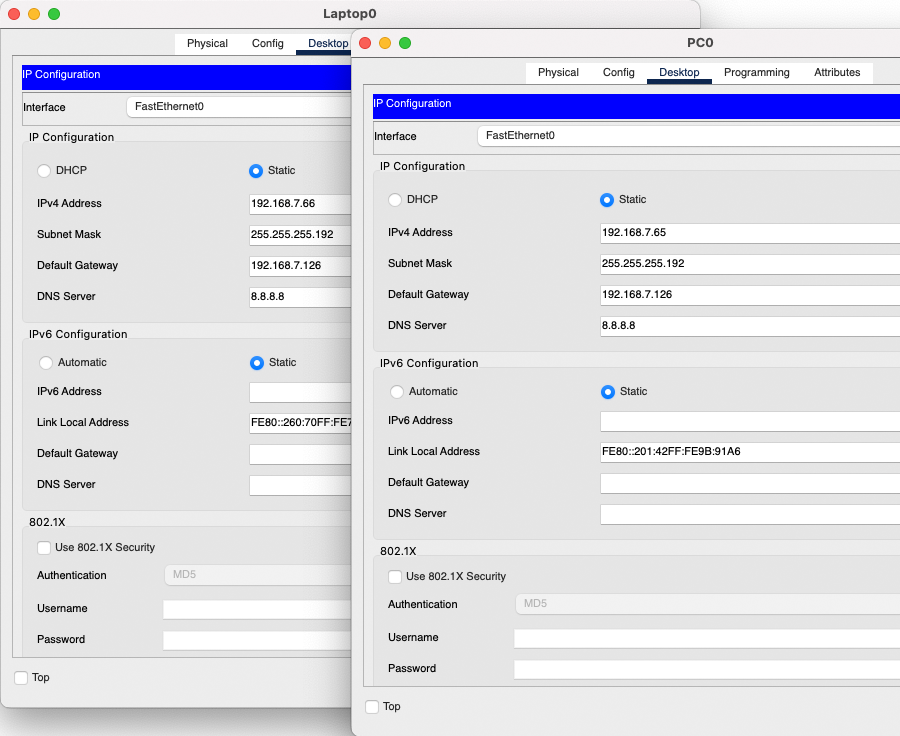
\includegraphics[scale=0.34 ,valign=c]{p2-connecting2lanswithrouter/Laptop0PC0_ip}        \\ \hline
                        And the same for Laptop1 and PC1.                                                                                                                                                                                                                                                                                                                                                           & 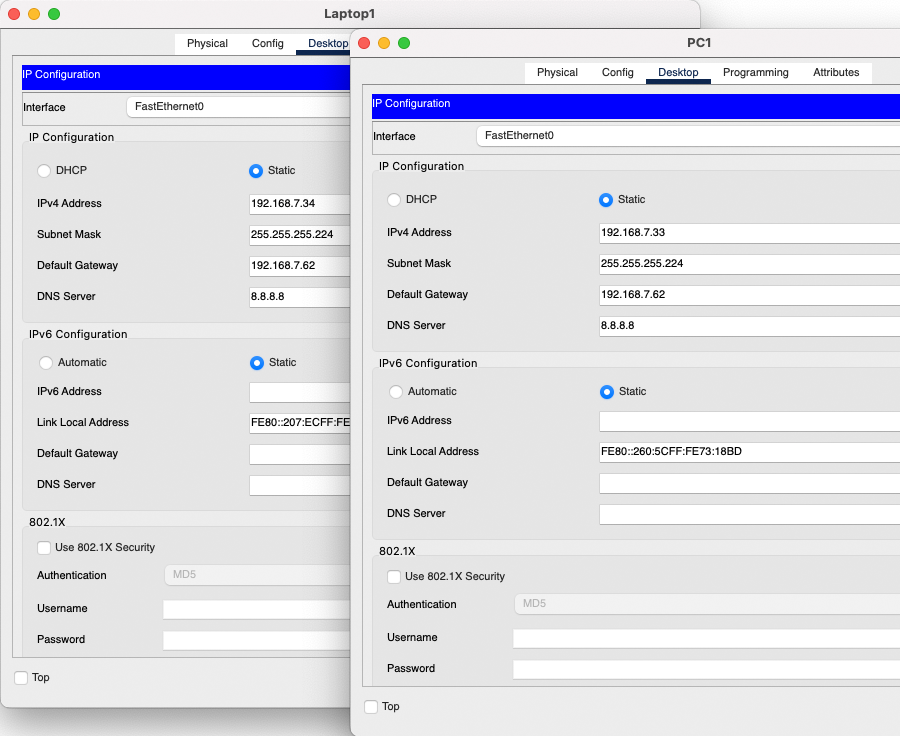
\includegraphics[scale=0.34 ,valign=c]{p2-connecting2lanswithrouter/Laptop1PC1_ip}        \\ \hline
                        For the router there's two options, both valid and exhibited in the report. The GUI in the right and the CLI, after this table, along CMD equivalent commands output. We're using \textbf{FastEthernet0/0} for \textit{LAN A} and \textbf{FastEthernet1/0} for \textit{LAN B}, going by the graphical user interface (GUI) it's crystal clear, just input the necessary IP and subnet mask. & 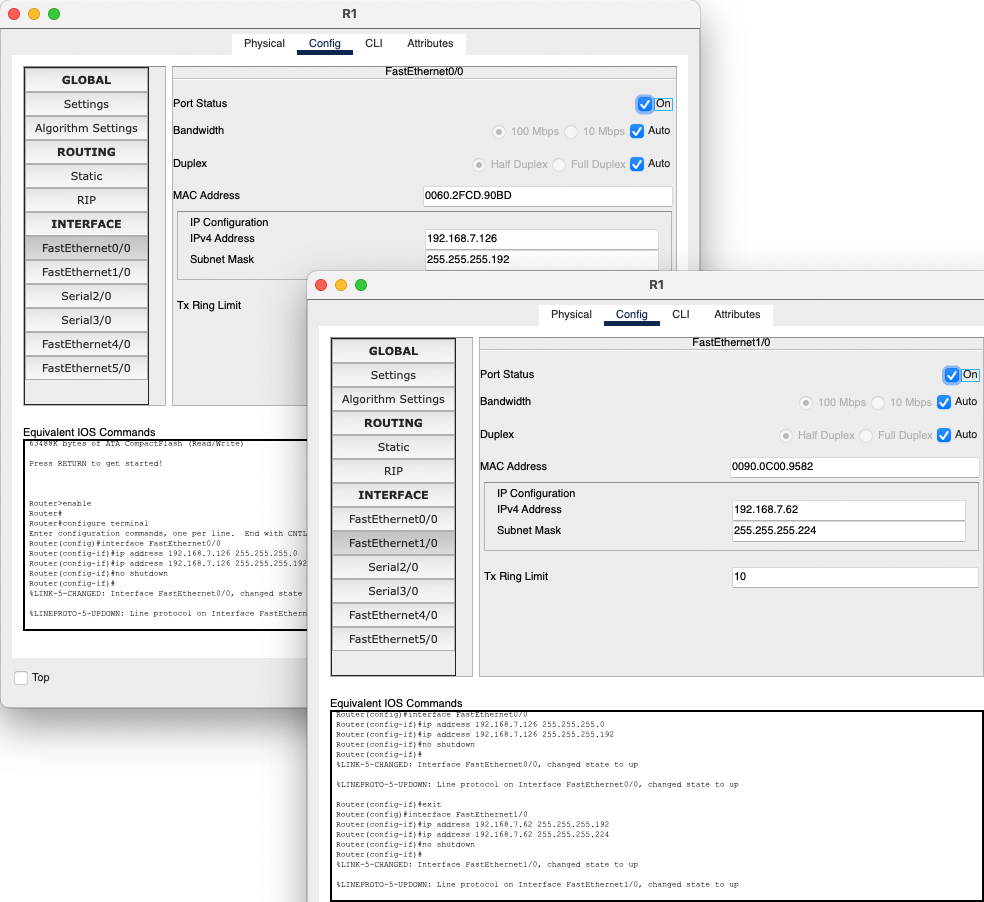
\includegraphics[scale=0.31 ,valign=c]{p2-connecting2lanswithrouter/R1-interfaces}        \\ \hline
                        To test the connection we select a device by \textbf{single-clicking} it (1), go to the \textit{desktop tab} (2) and select \textit{Command Prompt} (3).                                                                                                                                                                                                                                    & 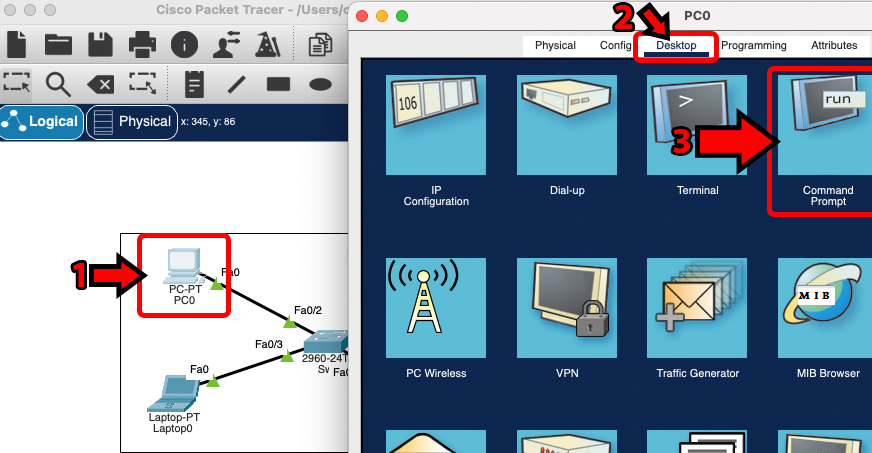
\includegraphics[scale=0.35 ,valign=c]{p1-connectingdevices/CiscoPacketTracer_cmdOutput}  \\ \hline
                        Contrary to our experiment in the previous section, it's unmistakable that after the first ping, the router provides information related to the whereabouts of the pinged device, due to \textbf{arp -a} command showing the router configured gateways.                                                                                                                                    & 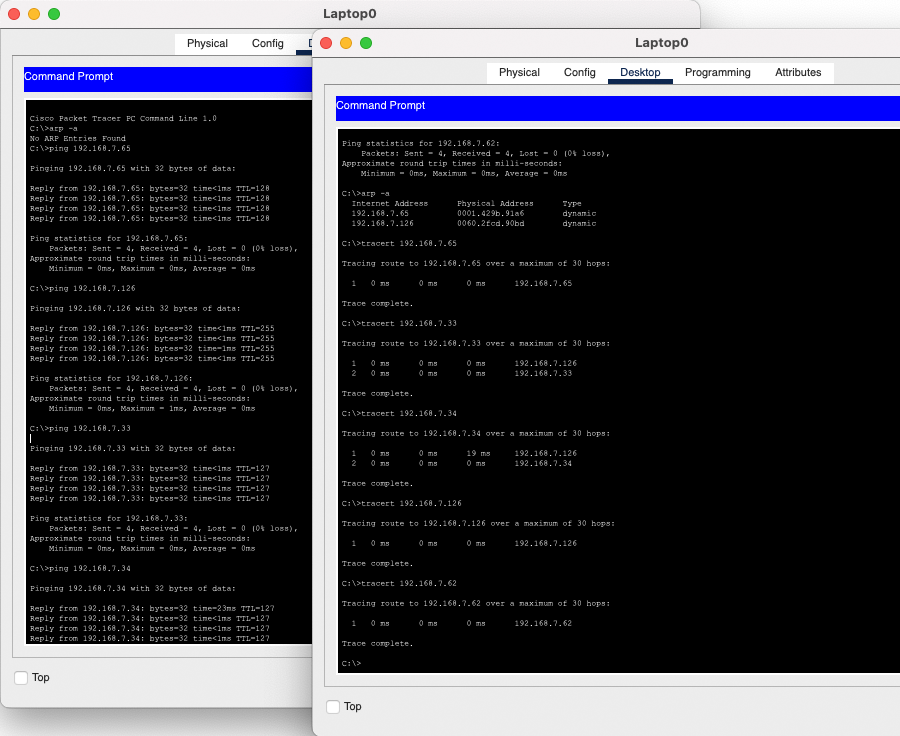
\includegraphics[scale=0.34 ,valign=c]{p2-connecting2lanswithrouter/Laptop0_cmdall}       \\ \hline
                        From the viewpoint of PC0.                                                                                                                                                                                                                                                                                                                                                                  & 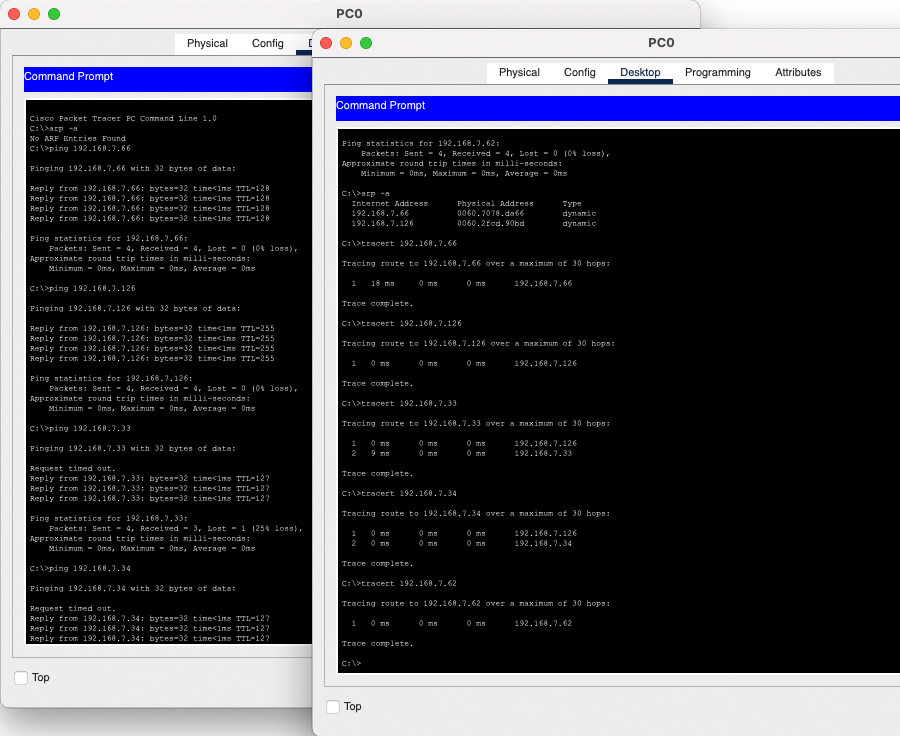
\includegraphics[scale=0.34 ,valign=c]{p2-connecting2lanswithrouter/PC0_cmdall}           \\ \hline
                        From the viewpoint of Laptop1.                                                                                                                                                                                                                                                                                                                                                              & 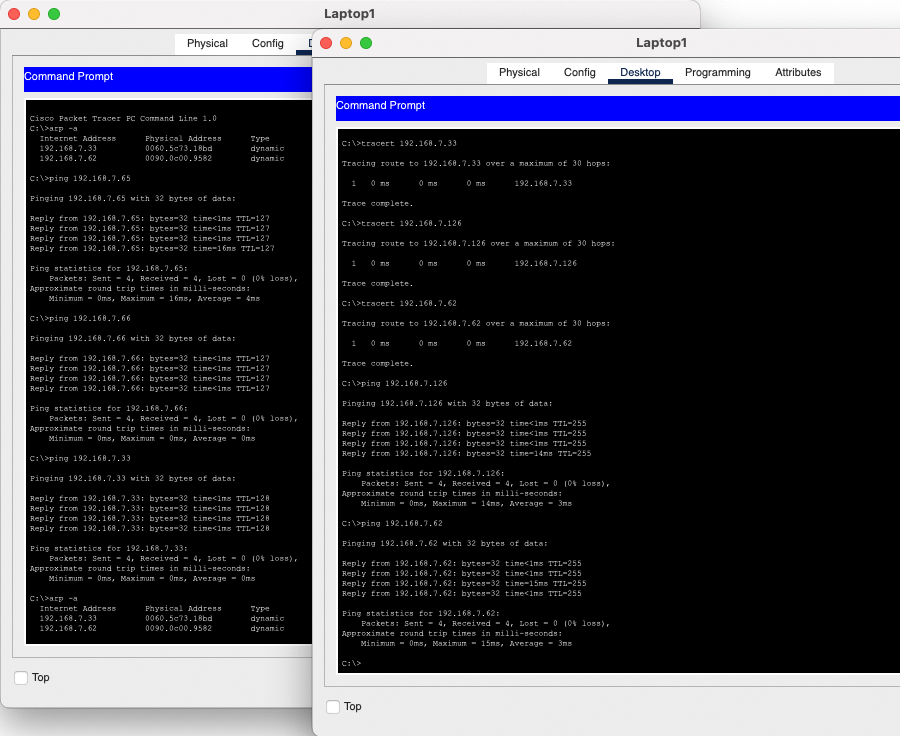
\includegraphics[scale=0.34 ,valign=c]{p2-connecting2lanswithrouter/Laptop1_cmdall}       \\ \hline
                        From the viewpoint of PC1.                                                                                                                                                                                                                                                                                                                                                                  & 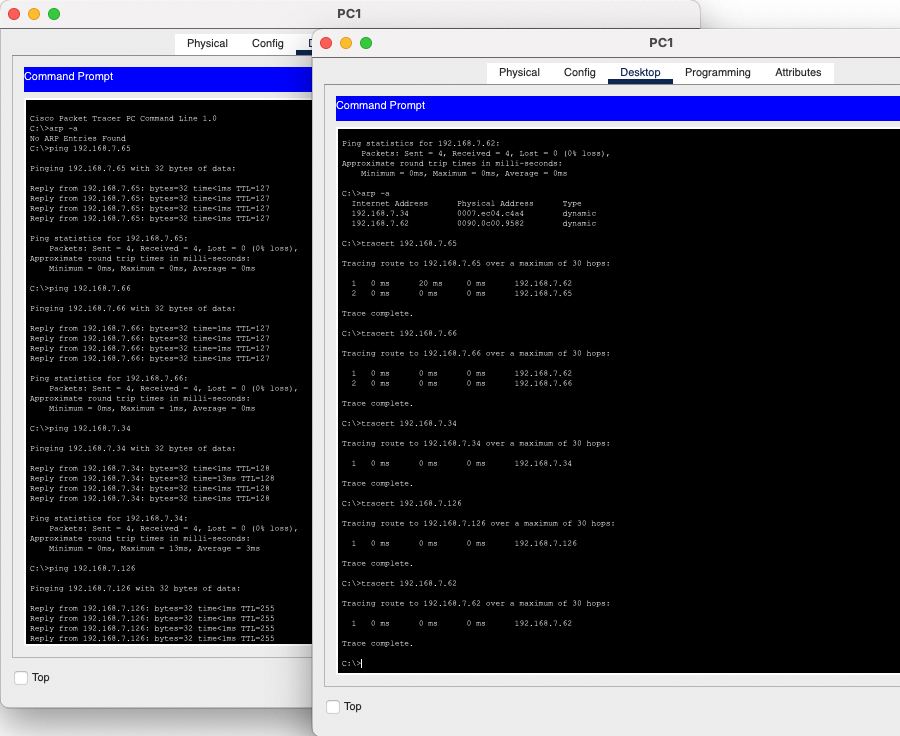
\includegraphics[scale=0.34 ,valign=c]{p2-connecting2lanswithrouter/PC1_cmdall}           \\ \hline
                        From the viewpoint of Router1.                                                                                                                                                                                                                                                                                                                                                              & 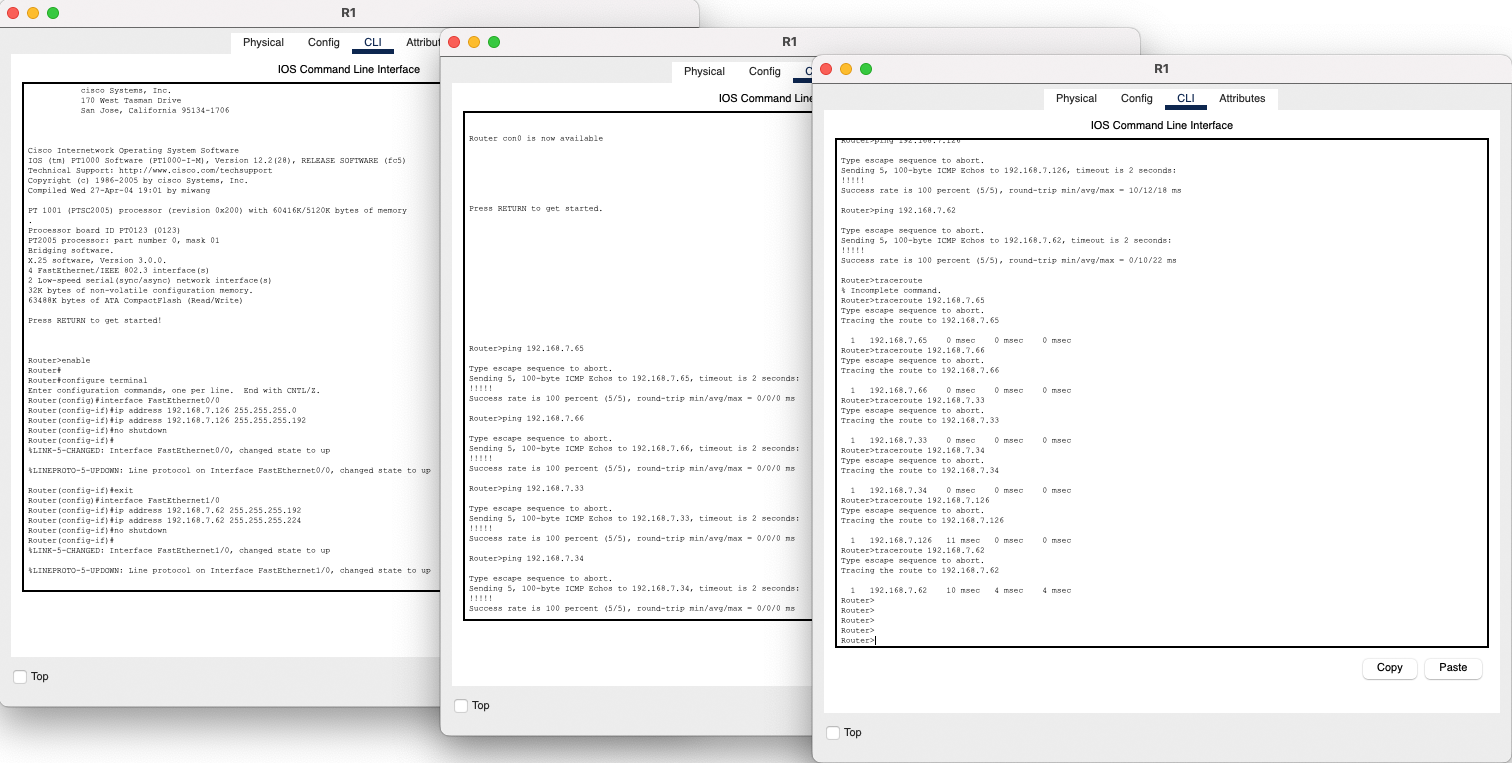
\includegraphics[scale=0.202,valign=c]{p2-connecting2lanswithrouter/R1-cliall}            \\ \hline

                        \caption{Cisco Packet Tracer guide}
                        \label{tab:cptg2}
                    \end{longtable}
                \end{center}
        \end{flushleft}

        And to supplement the output images, below are the text versions \textit{(considering this isn't a report for ants)}:
        \lstset{style=termoutputs}
        \lstinputlisting[
            language={},
            caption={PC0 CMD output},
            label={lst:pc0cmdoutp2}
        ]{./outputs/p2-connecting2lanswithrouter/PC0.txt}
        \lstinputlisting[
            language={},
            caption={Laptop0 CMD output},
            label={lst:laptop0cmdoutp2}
        ]{./outputs/p2-connecting2lanswithrouter/Laptop0.txt}
        \lstinputlisting[
            language={},
            caption={PC1 CMD output},
            label={lst:pc1cmdoutp2}
        ]{./outputs/p2-connecting2lanswithrouter/PC1.txt}
        \lstinputlisting[
            language={},
            caption={Laptop1 CMD output},
            label={lst:laptop1cmdoutp2}
        ]{./outputs/p2-connecting2lanswithrouter/Laptop1.txt}
        \lstinputlisting[
            language={},
            caption={Router 1 CLI output},
            label={lst:r1cmdoutp2}
        ]{./outputs/p2-connecting2lanswithrouter/R1.txt}

        It's evident why tracert is showing hops here. Now we have a router managing two local networks, as a consequence, each device goes through the router path.\\
        Ergo, the arp table is filled, not with device addresses but, with the router's network IP address.\\

        We're one step closer to become full network engineers!\\
        \begin{figure}[h]
            \centering
            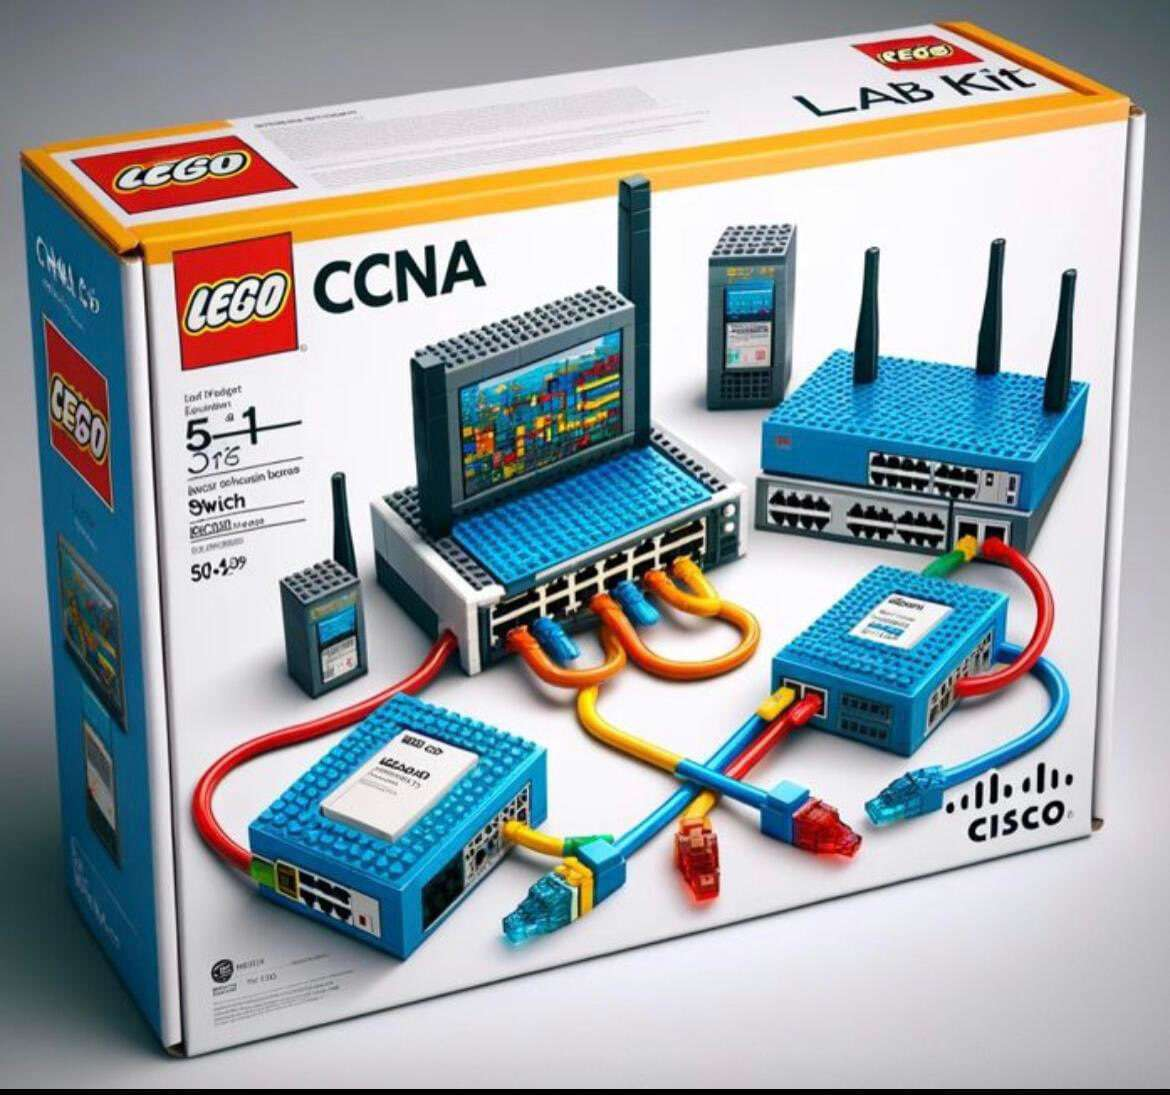
\includegraphics[scale=0.3]{ccna} 
            \caption{The best kind there is!}
            \label{fig:funnyccna}
        \end{figure}

%% Chapter: recomendations -----------------------------------------------------
\chapter{Issues and fixes}
    Cisco Packet Tracer in MacOS:\\
        \hspace*{10mm}No solution was found to deal with those annoying popups that takes primary focus over other windows, even using the latest version.

%% Chapter: conclusions --------------------------------------------------------
\chapter{Conclusions}
    By testing first with a switch we understood how arp tables work, storing it's information in devices since layered 2 equipments don't provide that functionality. Right after we got to put that argument to the test by using a router to connect to two distinct LANs. And it checks out, layered 3 devices store arp tables, displaying only their gateways through tracert (traceroute).

%% Bibliography ----------------------------------------------------------------
%\renewcommand{\bibname}{Bibliographic references}
%\bibliographystyle{chicago}
%\bibliography{refs}
%\addcontentsline{toc}{chapter}{\refname}  % add it to table of contents

%% Appendix --------------------------------------------------------------------
\appendix
\chapter{Appendix}
%%1}}}

\end{document}
